In questo capitolo verrà utilizzato il framework sviluppato in questa tesi e ne verranno valutate le performance, andando ad analizzare il comportamento di ogni fase al variare del numero di task e con configurazioni diverse.

\section{Infrastruttura di test}

Iniziamo descrivendo l'infrastruttura in cui sono stati effettuati i test, specificando le modalità di deployment dei componenti architetturali come NATS e wasmCloud.

\subsection{Ambiente Cloud}

Per la simulazione di un ambiente Cloud è stato utilizzato un cluster Kubernetes composto da tre nodi, implementati su macchine virtuali con sistema operativo Ubuntu 22.04, eseguite all'interno dell'hypervisor Proxmox. La distribuzione adottata è K3s, con una configurazione in cui ciascun nodo assume simultaneamente il ruolo di Master e Worker, garantendo così un'architettura distribuita e resiliente.\\
Sia wasmCloud che il cluster NATS sono stati installati utilizzando un Helm Chart, cioè un pacchetto pre-configurato di risorse Kubernetes. Il Chart è fornito direttamente da wasmCloud\footnote{wasmCloud Platform: \url{https://github.com/wasmCloud/wasmCloud/tree/main/charts/wasmcloud-platform}} e consente di deployare:
\begin{itemize}
    \item \textbf{Cluster NATS} configurabile con più repliche.
    \item \textbf{NATS-Box}, Pod utilizzabile per accedere al cluster NATS ed effettuare dei test di performance.
    \item \textbf{wasmCloud Operator}, consente di deployare le applicazioni definite nei manifest \texttt{wadm} anche tramite CLI Kubernetes (\texttt{kubectl}) utilizzando delle CRD.
    \item \textbf{WADM} componente dell'ecosistema wasmCloud che si occupa di ricevere le richieste di wash e istanziare i moduli in base alle specifiche dei manifest \texttt{wadm}.
    \item \textbf{wasmCloud Host}, creato sulla base di una configurazione custom di Kubernetes\texttt{wasmCloudHostConfig} e punto di esecuzione dei componenti Wasm. Possono esserne create più repliche se necessario.
\end{itemize}
L'infrastruttura viene mostrata nella Figura \ref{fig:wasmcloud_platform}, ottenuta tramite il cluster manager Rancher collegato al cluster Kubernetes.

\FloatBarrier
\begin{figure}[h]
    \centering
    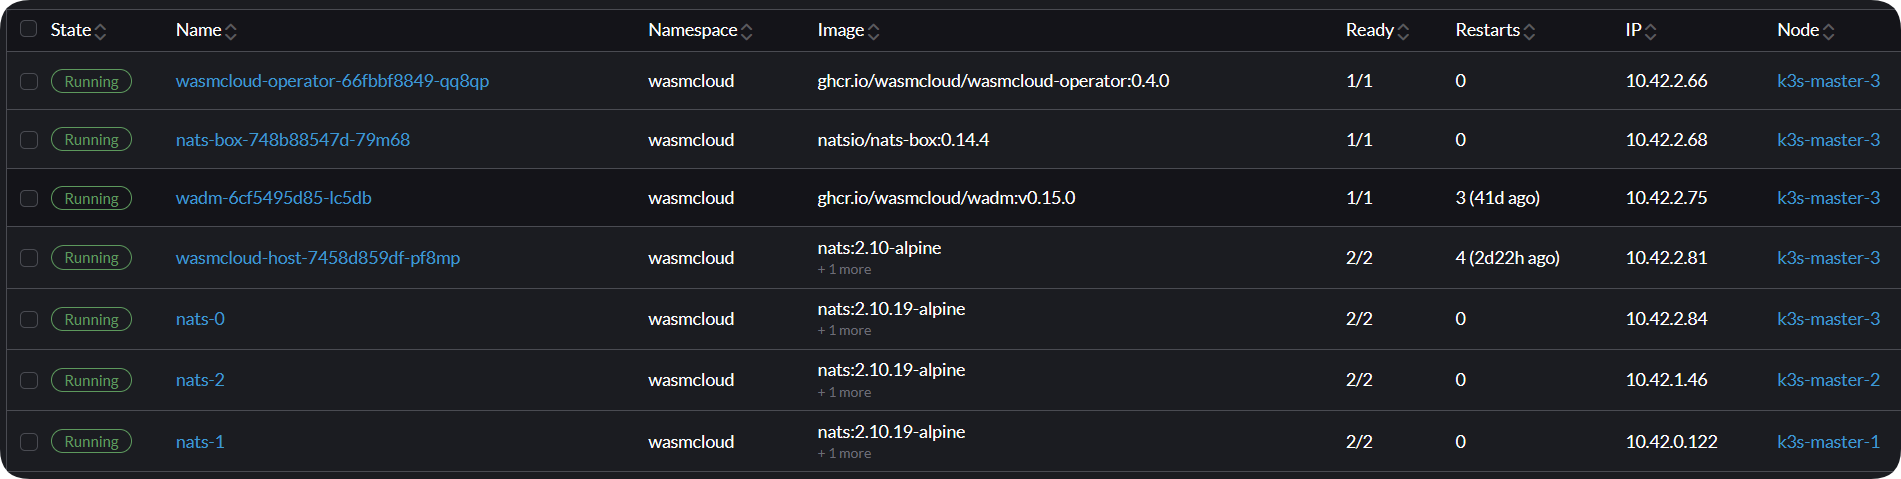
\includegraphics[width=\textwidth]{img/wasmcloud_platform_rancher.png}
    \caption{wasmCloud Platform su Kubernetes}
    \label{fig:wasmcloud_platform}
\end{figure}
\FloatBarrier


\subsection{Ambienti Edge}

Per simulare l'ambiente Edge sono stati utilizzati due semplici PC con sistema operativo Linux e provvisti di Docker Compose. L'host wasmCloud nei nodi Edge è stato deployato seguendo due modalità:
\begin{itemize}
    \item \textbf{Linux Service} istanziato tramite la wasmCloud Shell utilizzando il comando \lstinline{wash up -d --multi-local}.
    \item \textbf{Container} configurato tramite Docker Compose.
\end{itemize}

In entrambi i casi il collegamento con il cluster è stato effettuato utilizzando un nodo Leaf di NATS, deployato come container con la configurazione mostrata nel Listing \ref{code:nats_leaf_conf}.

\begin{lstlisting}[language=Python, caption={Configurazione nodo Leaf NATS}, captionpos=b, label={code:nats_leaf_conf}]
    jetstream {
      domain: leaf
    }
    leafnodes {
      remotes: [
        {
          url: "nats://nats.cluster.local:7422"     # Hostname del cluster NATS situato su Kubernetes
        }
      ]
    }
\end{lstlisting}

Per completare il flusso di esecuzione e simulare anche l'ambiente IoT sono stati utilizzati dei microcontrollori (come ESP32) collegati ai nodi Edge per produrre dati mock e metriche.\\
L'infrastruttura di test viene rappresentata nella Figura \ref{fig:infra_test} e può essere facilmente replicata grazie alle configurazioni presenti nella cartella \texttt{infra} del progetto.

\FloatBarrier
\begin{figure}[h]
    \centering
    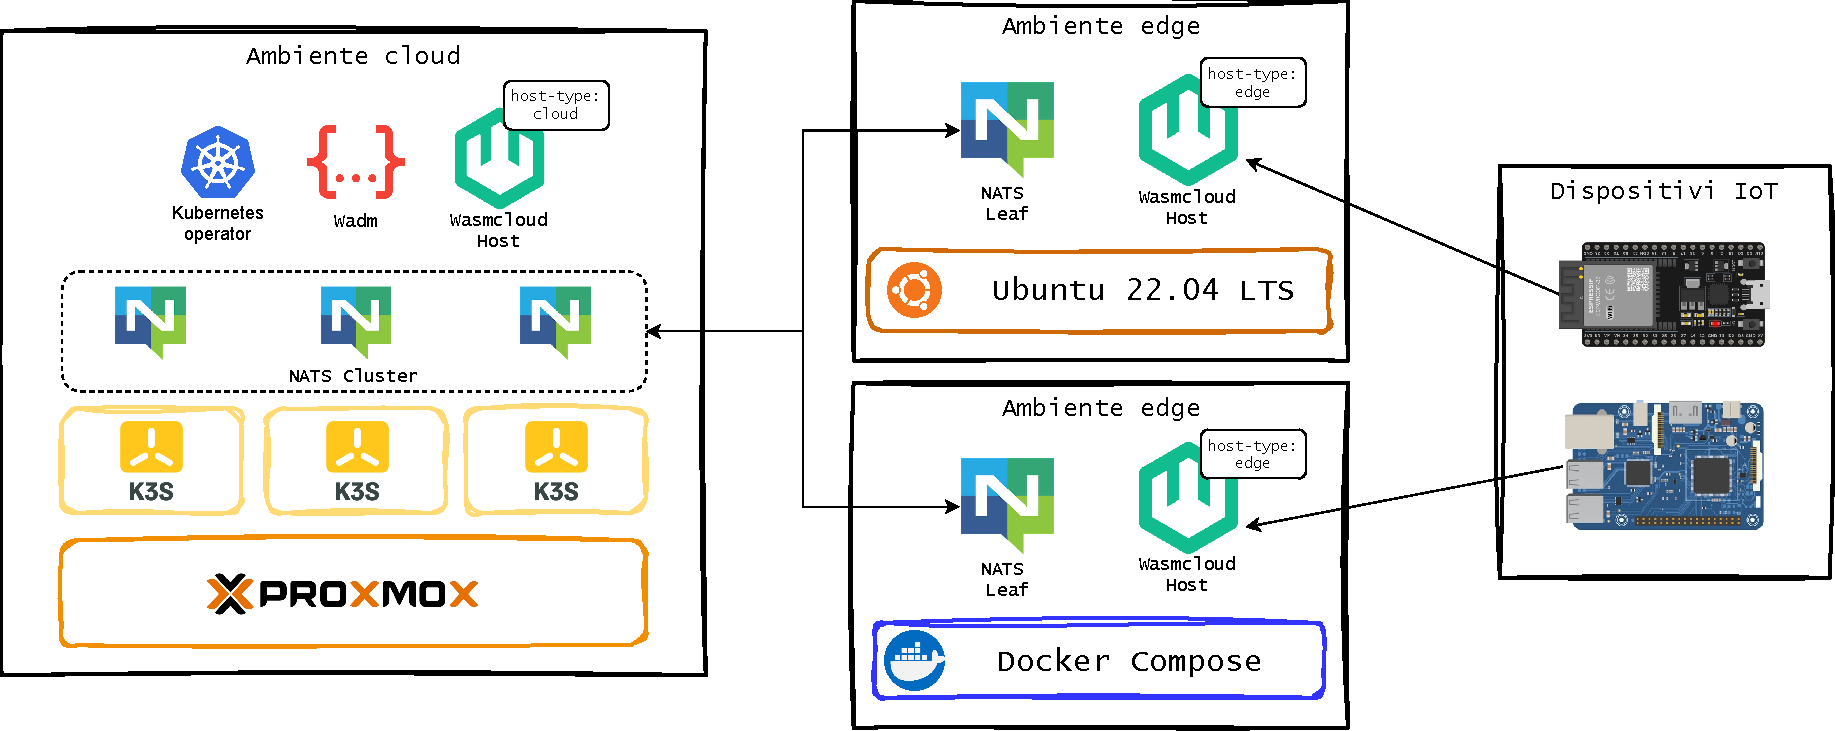
\includegraphics[width=\textwidth]{img/schemi/schemi-infrastuttura-impl.drawio.pdf}
    \caption{Infrastruttura di test}
    \label{fig:infra_test}
\end{figure}
\FloatBarrier

\subsection{Ambiente escuzione PELATO}

Il framework PELATO è stato eseguito all'interno di una delle macchine Edge. Per poter avere un'idea migliore delle performance del framework, riportiamo nel Listing \ref{code:hardware_spec} la configurazione hardware del PC in cui è stato eseguito.

\begin{lstlisting}[language=yaml, caption={Specifiche Hardware nodo Edge}, captionpos=b, label={code:hardware_spec}]
OS: Ubuntu 22.04 LTS x86_64 
Kernel: 6.11.0-17-generic
CPU: AMD Ryzen 7 7800X3D (8 cores 16 threads) 5.05 GHz
GPU: NVIDIA GeForce RTX 4070
Memory: 32 GiB DDR5 6000 MHz                                                        
\end{lstlisting}

Al momento della stesura di questo elaborato questa configurazione è considerabile high-end, quindi i grafici delle performance riportati nelle sezioni successive potrebbero essere ridimensionati in caso di esecuzione del framework in ambienti diversi, soprattutto nei casi di operazioni CPU-intensive come quella di build.

\section{Performance framework}

In questa sezione verranno mostrati i grafici e i risultati ottenuti sperimentando PELATO nell'infrastruttura descritta nella sezione precedente. Tutti i test che seguono sono stati misurati utilizzando la funzionalità di memorizzazione metriche integrata nel framework ed abilitabile con la variabile d'ambiente \texttt{ENABLE\_METRICS}. Inoltre, ogni test è stato eseguito almeno 5 volte e nei vari grafici viene riportato il confidence-interval al 95\% oltre al valore medio registrato.

\subsection{Startup Run}

Il primo test effettuato è stato quello di misurare la differenza nei tempi di esecuzione fra la prima volta e quelle successive: alla prima esecuzione del framework infatti dovrà anche buildare le immagini Docker utilizzate in fase di Build e Deploy.\\
Il test è stato effettuato lanciando PELATO su una configurazione di progetto minimale, con una singola task e codice con alcuna libreria aggiuntiva. Di seguito vengono riportati i grafici ottenuti analizzando le metriche della fase Build (Figura \ref{fig:test_startup_build}) e di quella Deploy (Figura \ref{fig:test_startup_deploy}). Sono state omesse le metriche della fase di Generazione in quanto non vi è alcuna differenza in quel caso fra la prima esecuzione e quelle successive.

\FloatBarrier
\begin{figure}[h]
    \centering
    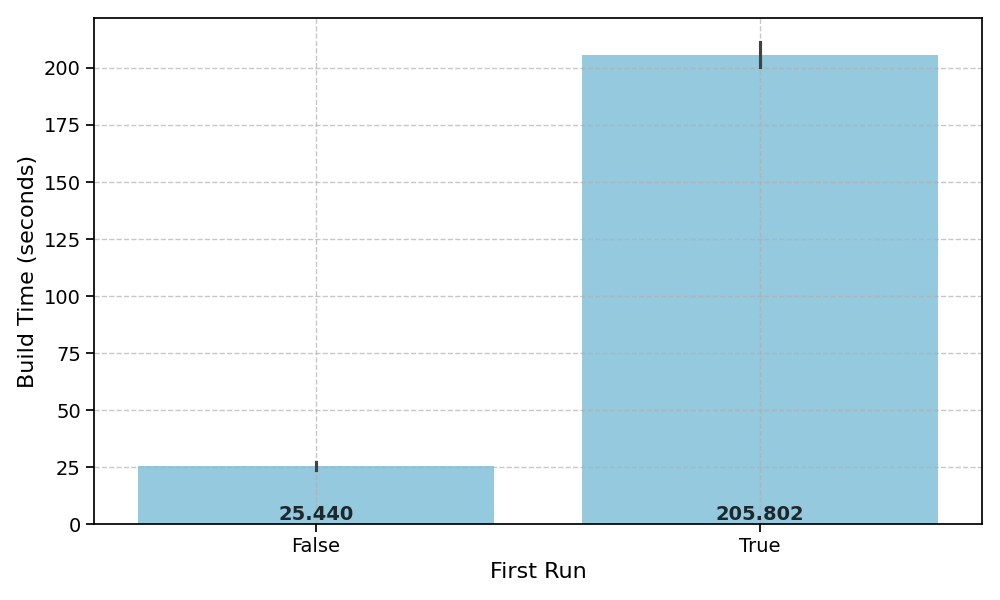
\includegraphics[width=0.9\textwidth]{img/plots/barplot_startup_build.png}
    \caption{Tempo impiegato per la prima esecuzione di Build}
    \label{fig:test_startup_build}
\end{figure}
\FloatBarrier

Come è possibile vedere nella Figura \ref{fig:test_startup_build} i tempi di esecuzione cambiano drasticamente: il framework impiega circa 175 secondi aggiuntivi per buildare l'immagine \texttt{wash-build-image}, utilizzata nella fase di Build del componente Wasm. Questo comportamento è atteso, infatti l'immagine deve contenere tutti gli strumenti per compilare il progetto Wasm ed è necessario del tempo per poterli installare.

\FloatBarrier
\begin{figure}[h]
    \centering
    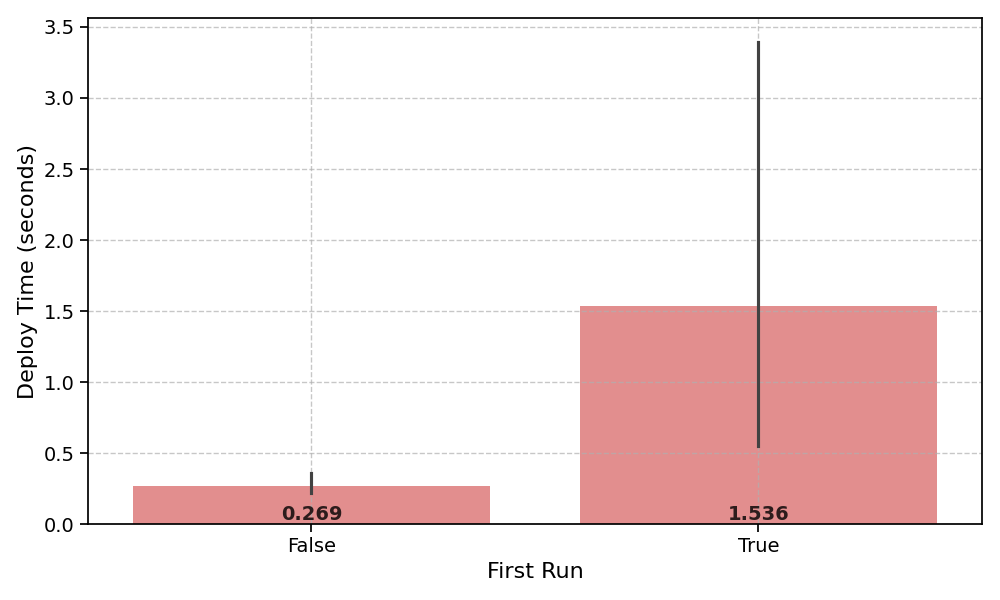
\includegraphics[width=0.9\textwidth]{img/plots/barplot_startup_deploy.png}
    \caption{Tempo impiegato per la prima esecuzione di Deploy}
    \label{fig:test_startup_deploy}
\end{figure}
\FloatBarrier

Un risultato più interessante è quello mostrato nella Figura \ref{fig:test_startup_deploy}: infatti il tempo di creazione dell'immagine \texttt{wash-deploy-image} è pressoché nullo. Questo è riconducibile alle ottimizzazioni effettuate dal Docker engine, infatti i layer dell'immagine precedentemente buildata \texttt{wash-build-image} rimangono in cache e vengono riutilizzati per costruire quella di deploy, che contiene esclusivamente il tool wash, riducendo drasticamente i tempi di esecuzione.

\subsection{Esecuzione parallela o sequenziale}

Il secondo test effettuato riguarda la differenza di performance fra le modalità di istanziamento dei container, cioè sequenziale o parallela. Le performance vengono misurate utilizzando il tempo di esecuzione per ogni fase.

\FloatBarrier
\begin{figure}[ht!]
    \centering
    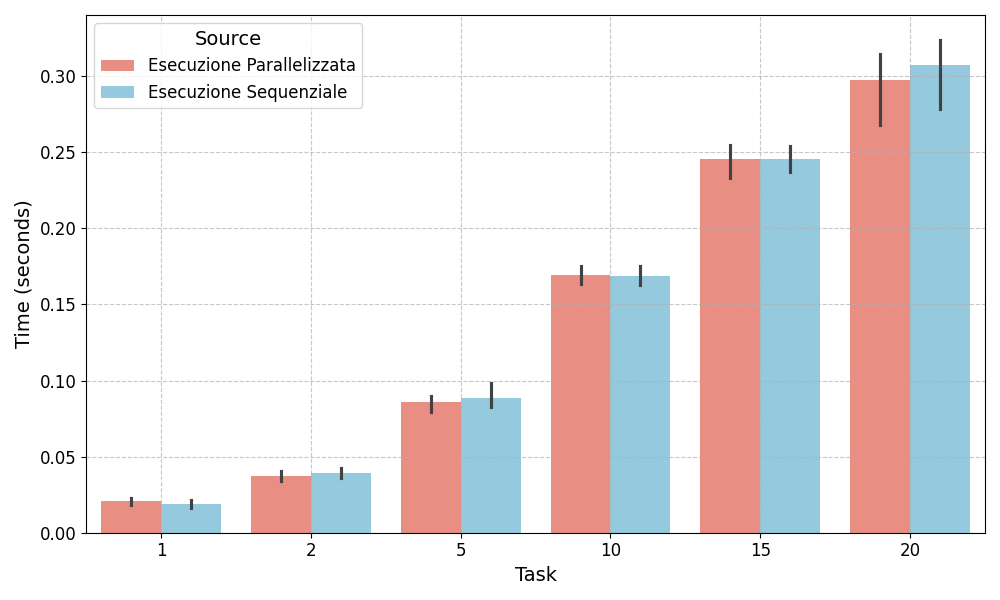
\includegraphics[width=0.9\textwidth]{img/plots/gen_time_paired_barplot.png}
    \caption{Generazione codice sequenziale vs parallela}
    \label{fig:test_seq_par_gen}
\end{figure}
\FloatBarrier

\FloatBarrier
\begin{figure}[ht!]
    \centering
    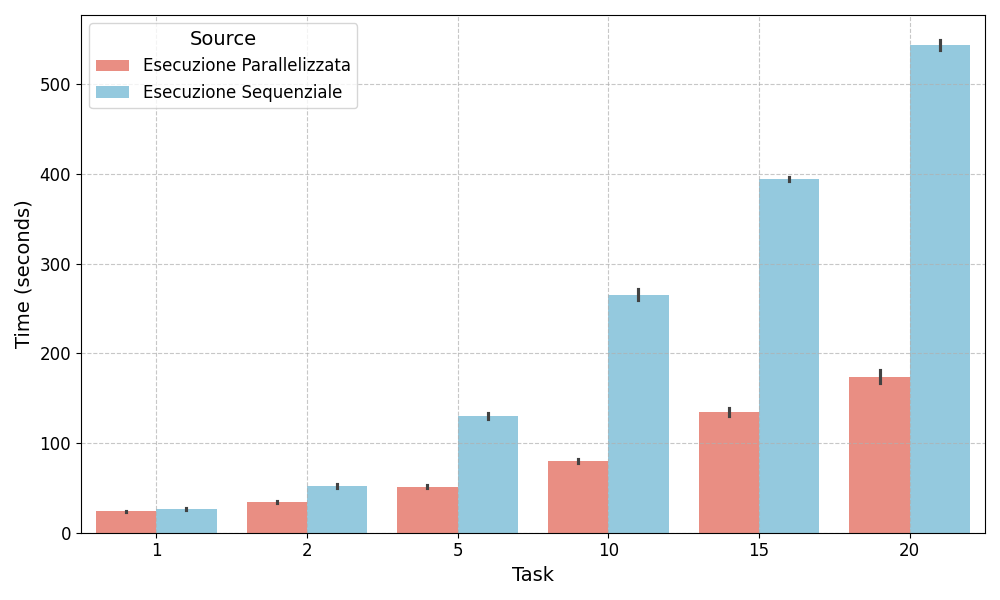
\includegraphics[width=0.9\textwidth]{img/plots/build_time_paired_barplot.png}
    \caption{Build sequenziale vs parallela}
    \label{fig:test_seq_par_build}
\end{figure}
\FloatBarrier

\FloatBarrier
\begin{figure}[ht!]
    \centering
    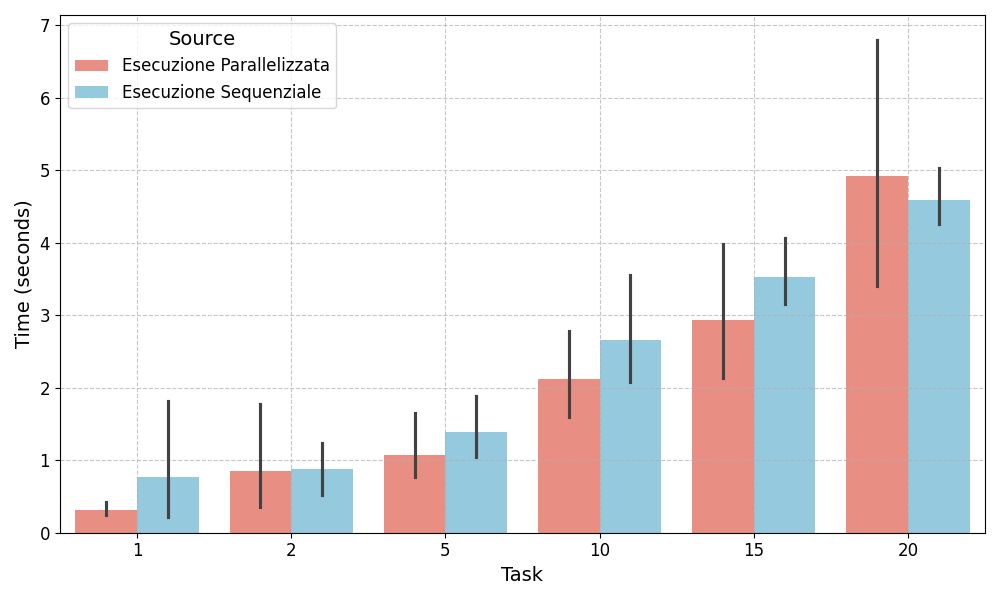
\includegraphics[width=0.9\textwidth]{img/plots/deploy_time_paired_barplot.png}
    \caption{Deployment sequenziale vs parallela}
    \label{fig:test_seq_par_deploy}
\end{figure}
\FloatBarrier

\FloatBarrier
\begin{figure}[ht!]
    \centering
    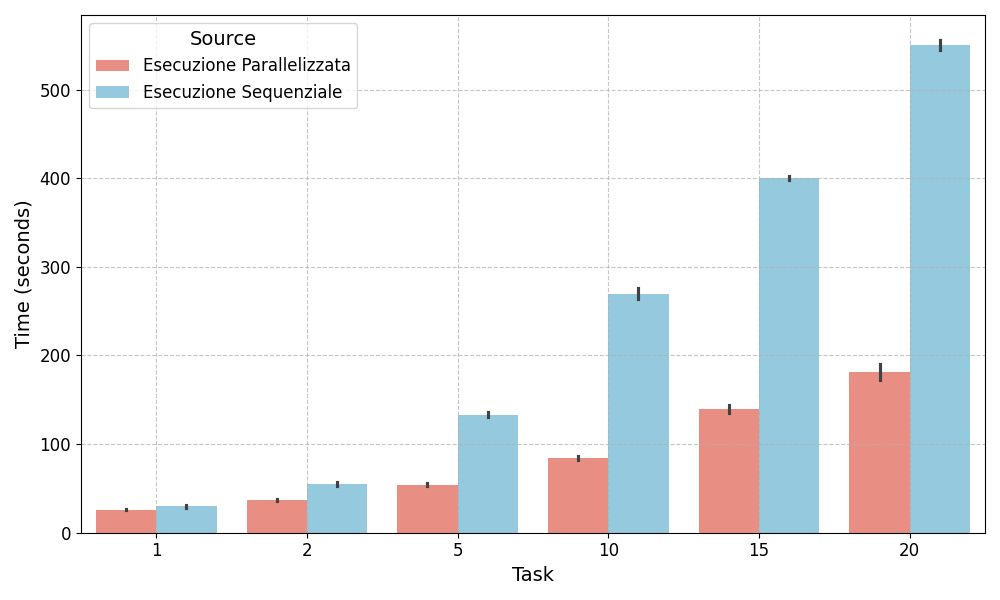
\includegraphics[width=0.9\textwidth]{img/plots/total_time_paired_barplot.png}
    \caption{Pipeline PELATO sequenziale vs parallela}
    \label{fig:test_seq_par_total}
\end{figure}
\FloatBarrier

Analizziamo il comportamento del framework in base alle modalità:
\begin{itemize}
    \item Possiamo notare nella Figura \ref{fig:test_seq_par_gen} come la fase di Generazione non sia influenzata dalla modalità, comportamento atteso dato che non fa utilizzo dei container.
    \item La fase di Build è quella in cui è più evidente il vantaggio della parallelizzazione: sebbene la differenza sia poca per un numero di task basso, essa cresce esponenzialmente man mano che il numero sale, arrivando ad un tempo di esecuzione tre volte più basso rispetto alla modalità sequenziale, come mostrato nella Figura \ref{fig:test_seq_par_build}.
    \item Nella fase di Deploy si può notare un lieve miglioramento nella modalità parallelizzata, con una piccola discrepanza per n-task = 20 probabilmente dovuta ad un problema di connettività. Questo è osservabile nella Figura \ref{fig:test_seq_par_deploy}.
\end{itemize}

Osservando la Figura \ref{fig:test_seq_par_total}, che raffigura il tempo di esecuzione totale, possiamo osservare come la modalità parallelizzata sia in tutte le situazioni la scelta più efficiente e che sfrutta al meglio le risorse della macchina.

\subsection{Differenze fra template}

Durante la sperimentazione è emersa una leggera differenza nei tempi di esecuzione della pipeline in base al template scelto come base per i vari Task del file workload. Di seguito vengono riportati i grafici che paragonano i tempi di esecuzione del framework in base ai due template:
\begin{itemize}
    \item \texttt{processor\_nats}: utilizza esclusivamente il provider NATS.
    \item \texttt{http\_producer\_nats}: utilizza il provider NATS e anche il provider del web server HTTP.
\end{itemize}
Come si può vedere dalle figure \ref{fig:test_provider_gen}, \ref{fig:test_provider_build} e \ref{fig:test_provider_deploy}, i tempi di esecuzione sono leggermente più alti per il template con entrambi provider. Questo risultato è conforme alle aspettative, in quanto effettuare operazioni su più componenti risulta più oneroso per ogni parte della pipeline. Il risultato finale mostrato in Figura \ref{fig:test_provider_total} lo conferma.

\FloatBarrier
\begin{figure}[ht!]
    \centering
    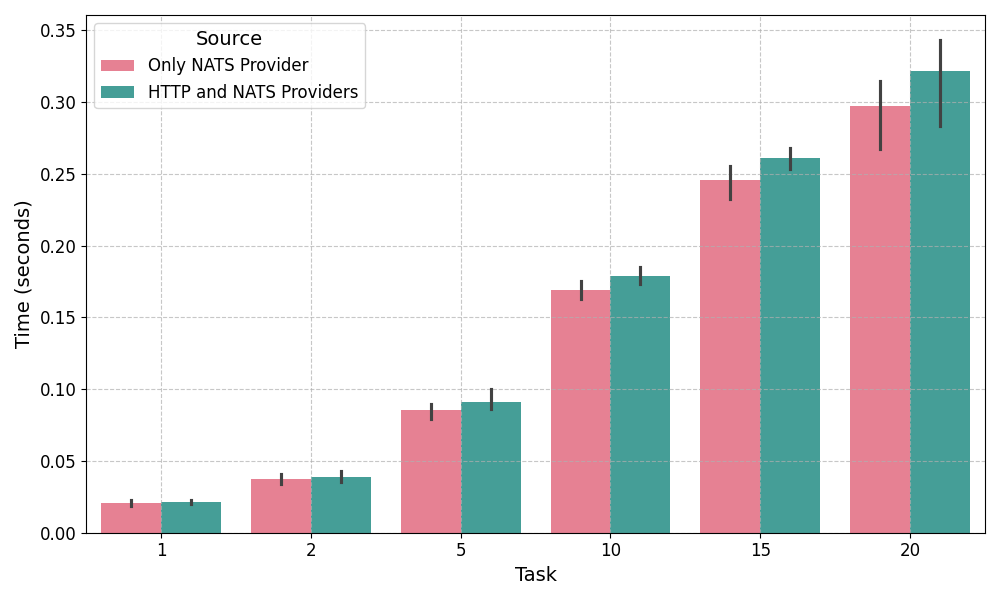
\includegraphics[width=0.9\textwidth]{img/plots/gen_time_providers_barplot.png}
    \caption{Generazione codice, differenze fra template}
    \label{fig:test_provider_gen}
\end{figure}
\FloatBarrier

\FloatBarrier
\begin{figure}[ht!]
    \centering
    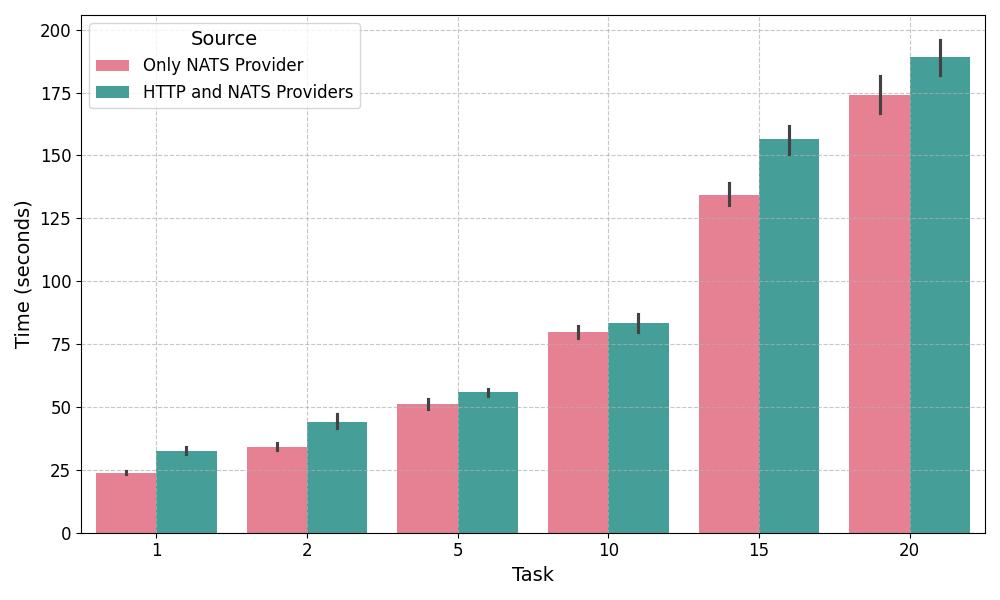
\includegraphics[width=0.9\textwidth]{img/plots/build_time_providers_barplot.png}
    \caption{Build, differenze fra template}
    \label{fig:test_provider_build}
\end{figure}
\FloatBarrier

\FloatBarrier
\begin{figure}[ht!]
    \centering
    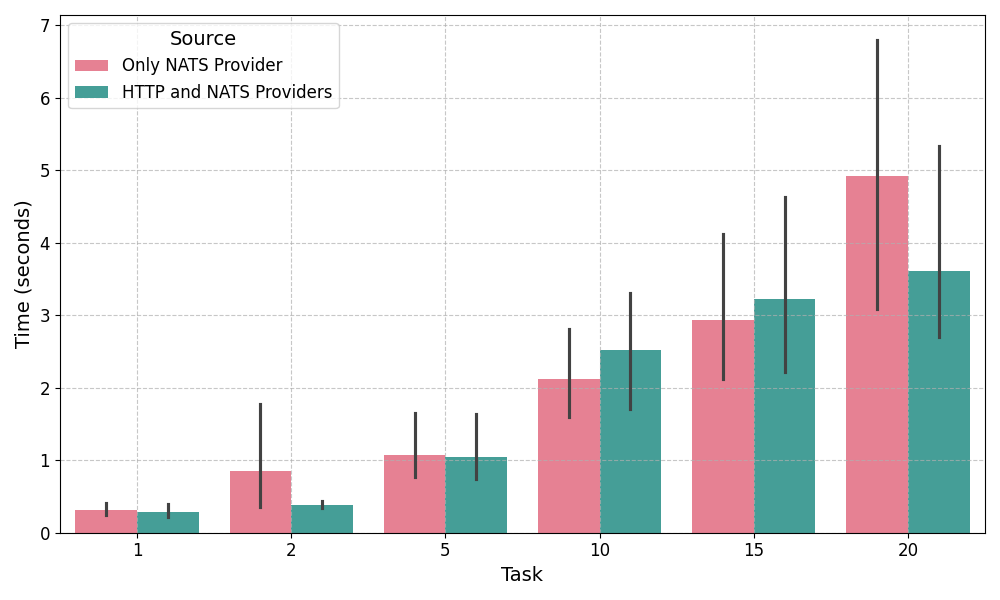
\includegraphics[width=0.9\textwidth]{img/plots/deploy_time_providers_barplot.png}
    \caption{Deployment, differenze fra template}
    \label{fig:test_provider_deploy}
\end{figure}
\FloatBarrier

\FloatBarrier
\begin{figure}[ht!]
    \centering
    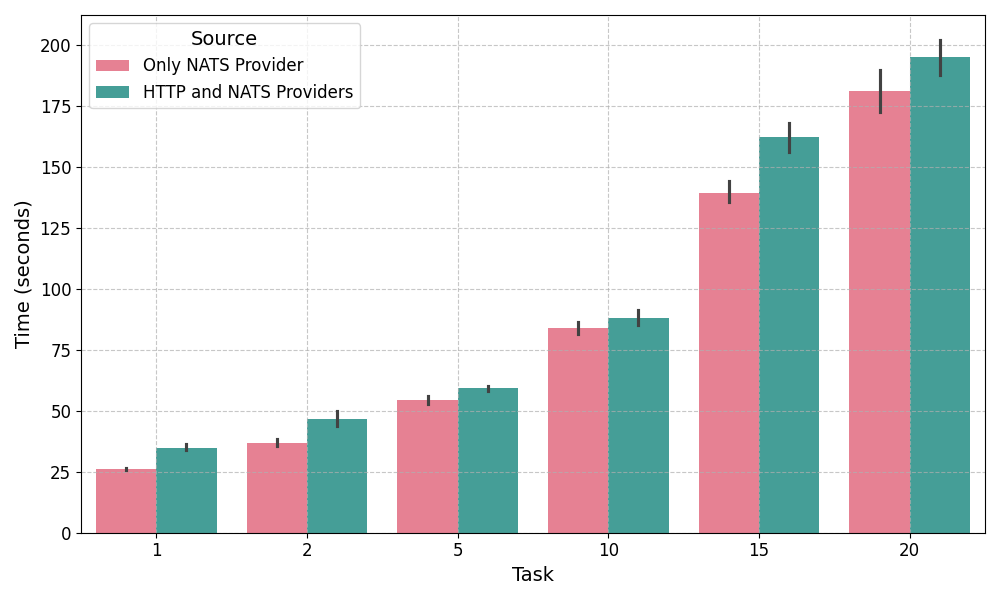
\includegraphics[width=0.9\textwidth]{img/plots/total_time_providers_barplot.png}
    \caption{Pipeline PELATO, differenze fra template}
    \label{fig:test_provider_total}
\end{figure}
\FloatBarrier

\subsection{Criticità}

In questa sezione verranno riportate le criticità riscontrate durante la fase di testing. Le prime discrepanze, come già accennato in una sezione precedente, appaiono durante l'analisi delle metriche della fase di Deploy. In alcuni casi i tempi di deployment delle applicazioni si scostano dalle previsioni (anche se di pochi secondi), probabilmente per problemi dovuti al sovraccarico della rete o del componente WADM del cluster wasmCloud.\\
Una criticità più importante è apparsa durante il test di esecuzione del framework in modalità parallelizzata con n-task \(\geq\) 15. Talvolta infatti l'esecuzione fallisce e la libreria di Docker restituisce la seguente eccezione
\begin{lstlisting}
     UnixHTTPConnectionPool(host='localhost', port=None): Read timed out. (read timeout=60)
\end{lstlisting}
probabilmente dovuta ad un sovraccarico della Unix Socket utilizzata da Docker. Per tamponare il problema è possibile aumentare il timeout della socket utilizzando le seguenti variabili d'ambiente
\begin{lstlisting}
DOCKER_CLIENT_TIMEOUT=120
COMPOSE_HTTP_TIMEOUT=120
\end{lstlisting}
e riavviando il servizio di Docker.

\section{Test Failover wasmCloud}

In questa sezione viene effettuato un test di recovery dopo il fallimento di un nodo. Lo scenario è composto da:
\begin{itemize}
    \item Cluster wasmCloud in un ambiente Cloud. Il wasmCloud Host è dotato di label \texttt{host-type: cloud}.
    \item Due ambienti Edge in reti separate, dotati di wasmCloud Host con label \texttt{host-type: edge}.
\end{itemize}

Il framework PELATO è stato usato per deployare un'applicazione che espone un web server HTTP (template http\_producer\_nats) utilizzando i file di configurazione mostrati nei Listing \ref{code:workflow_file_test} e \ref{code:task_file_test}, che descrivono un semplice use-case di un componente che riceve delle misurazioni della temperatura di una stanza tramite richieste HTTP, le converte da Celsius a Kelvin le pubblica su NATS. 

\begin{lstlisting}[language=yaml, caption={Workflow test recovery}, captionpos=b, label={code:workflow_file_test}, keepspaces=true]
project_name: Temperature data analysis
tasks:
  - name: Temp data conversion
    type: http_producer_nats
    code: convert.go
    targets:
      - edge
    source_topic: living_room_celsius_data
    dest_topic: living_room_kelvin_data
    component_name: celsius_to_kelvin_conversion
    version: 1.0.0
\end{lstlisting}

\begin{lstlisting}[language=Go, caption={Task file test recovery}, captionpos=b, label={code:task_file_test}, keepspaces=true]
    package main
    import (
    	"encoding/json"
    )
    type Request struct {
        Data float64
        Name string
    }
    func exec_task(arg string) string{
        req := Request{}
    	json.Unmarshal([]byte(arg), &req)
    	// Conversion between celsius and kelvin
    	req.Data = req.Data + 273.15
    	// return the json string
    	json, _ := json.Marshal(req)
    	return string(json)
    }
\end{lstlisting}

Il test effettuato vuole simulare la caduta di uno dei due nodi Edge (schematizzato in Figura \ref{fig:test_recovery}) e misurare il tempo impiegato dall'infrastruttura wasmCloud per accorgersi del problema e spostare l'esecuzione dell'applicazione sul nodo Edge funzionante.

\FloatBarrier
\begin{figure}[ht!]
    \centering
    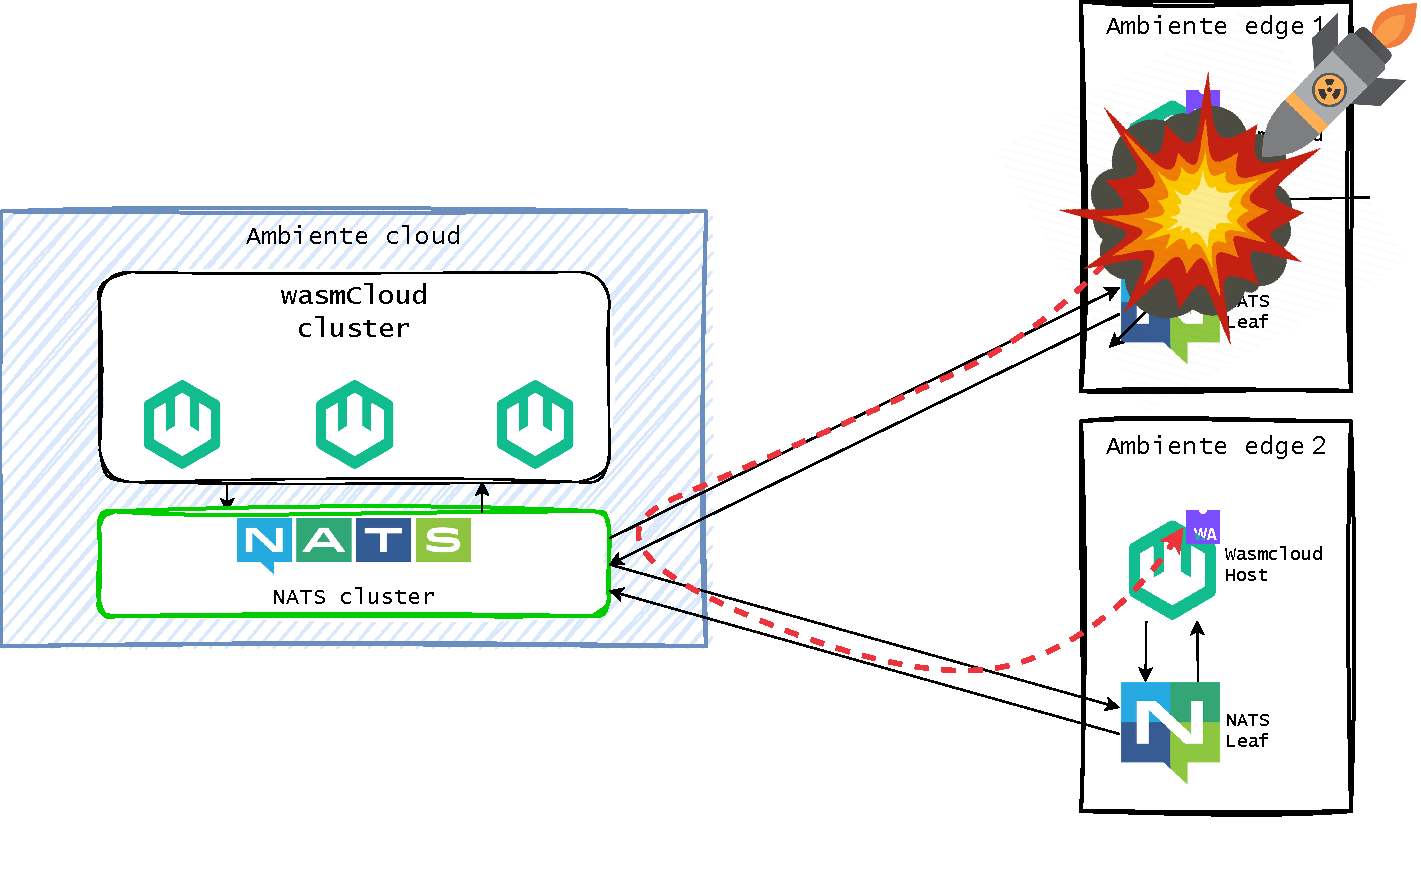
\includegraphics[width=0.75\textwidth]{img/schemi/schemi-test-failover-good.drawio.pdf}
    \caption{Scenario test failover}
    \label{fig:test_recovery}
\end{figure}
\FloatBarrier

I dati sono stati ottenuti misurando il tempo passato dalla distruzione del nodo 1 al deployment dell'applicazione sul nodo 2. L'applicazione viene considerata correttamente deployata quando il server HTTP risponde alla chiamata di test effettuata. Il nodo è stato cancellato stoppando il container in cui veniva eseguito il wasmCloud Host, la misurazione è stata effettuata tramite uno script bash che lancia comandi curl fino ad ottenere una risposta.\\
Dopo aver effettuato 5 test, il tempo di recovery si è assestato sui \(23 \pm 1.5\) secondi (come è possibile osservare dalla Figura \ref{fig:test_recovery_plot}), dimostrando come l'infrastruttura basata su wasmCloud possa rispondere alle perdite in tempi brevi.

\FloatBarrier
\begin{figure}[ht!]
    \centering
    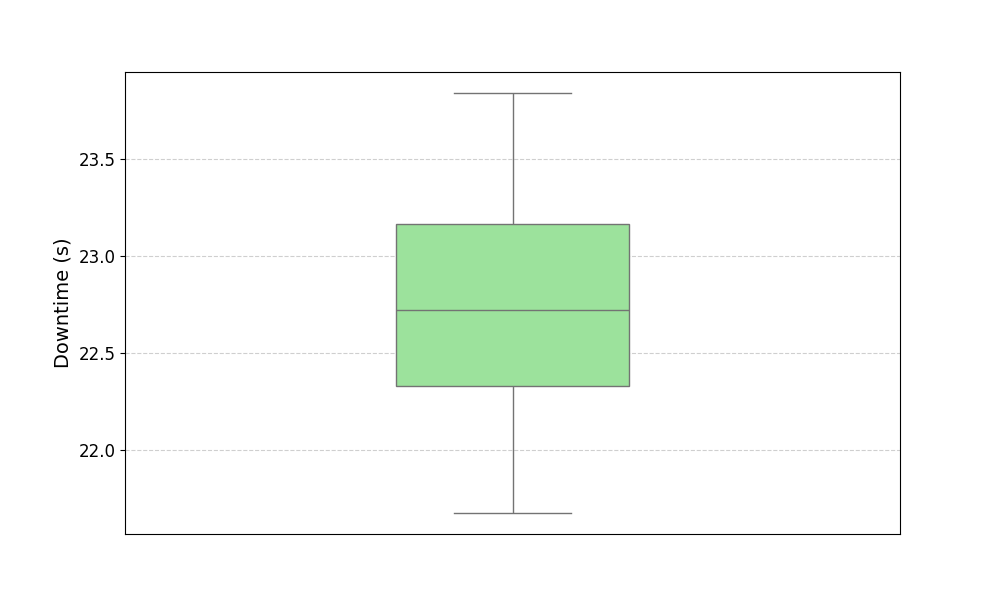
\includegraphics[width=0.75\textwidth]{img/plots/boxplot_failover.png}
    \caption{Tempo di recovery wasmCloud}
    \label{fig:test_recovery_plot}
\end{figure}
\FloatBarrier